\chapter{Linking Media events and Twitter events}
\section{Introduction}
\section{Related Work}

The task of discovering joint events from news streams including both social and mainstream media has received little attention in the recent literature. In this section, we review existing works on similar tasks: aligning social-media contents with parts or paragraphs of a longer text, matching a tweet with a relevant news article, retrieve tweets related to a news article and, finally, jointly discover events from heterogeneous streams of documents.

\subsection{Social content alignment}
\label{Social content alignment}
A first way of linking tweets and news is to associate to each part of a text the corresponding tweets (that are considered as comments or reactions to this specific part). \cite{hu_et-lda:_2012} develop ET-LDA, a Bayesian model that jointly extract topics from a text and a collection of tweets, and perform text segmentation. A segment may consist of one or several paragraphs, and each segment discusses a set of topics. Tweets are "aligned" with one segment if most of their words belong to one of the topics of this segment. Conversely, they are defined as "general tweets" if most of their words belong to general topics. The model is tested on two texts: a speech by President Obama and the transcript of a 2011 Republican Primary debate. The tweets are collected using hashtags (``\#MESpeech" and ``\#ReaganDebate") that unambiguously relate to these events. 

\subsection{Match tweets-articles pairs}
\label{Match tweets-articles pairs}
Another related task consists in finding, for a given tweet, the most relevant news article. This research area aims at providing more context for the reader of a tweet, or for an automatic NLP tool. \cite{guo_linking_2013} propose a graph-based latent variable model that extracts text-to-text correlations via hashtags and named entities in order to enrich the sense of a short text and help to identify the most related article. They also introduce a dataset of articles from CNN and the New York Times and of tweets containing a link to one of these media outlets. The tweet-news pairs are identified by matching urls, but "trivial" pairs (when the tweet contains exactly the title of the article) are removed from the dataset.

\cite{zhao_interactive_2019} use an interactive attention deep neural network in order to learn new representations of source and target texts. The representation of the source text is enriched with the target text, considered as the neighbor information or the context of the source text, and vice-versa. Mutual  differences  between  the  original  and  the  new representation are used to produce a similarity score. The model is tested on several applications, including the tweet-article matching task defined by \cite{guo_linking_2013}.

Compared to \cite{guo_linking_2013}, \cite{danovitch2020linking} is interested in the reverse task: given a news article, find the most relevant tweet (though their architecture seems to be symmetrical and could probably be used for both tasks). They use a deep neural attention network with a Siamese architecture\footnote{See section \ref{embedding_phrases} for a definition of a Siamese network} to jointly embed tweet/article pairs. They address the problem of the decreasing weight of tokens with article length in attention-based architectures by using a sparse activation function \citep{peters2019sparse}. They also use Star-Transformer \citep{guo2019star}, a lightweight alternative to the fully-connected Transformer architecture \citep{vaswani2017attention} that reduces its complexity from quadratic to linear time. The model is trained with triplet loss. At inference time, this architecture produces embeddings for tweets and articles, allowing to perform distance computations using cosine similarity.

\subsection{Social content retrieval}
\label{Social content retrieval}
Several articles \citep{tsagkias_linking_2011, tanev_enhancing_2012, suarez2018data} address the task of linking traditional media and social media as an Information Retrieval problem, which can be formulated as follows: given a news article, find social media posts that reference it. In this approach, there is no notion of completeness of the retrieved data: these algorithms are often evaluated without taking the ``size" of the event (in terms of total number of generated documents) into account. On the other hand, the order of the results is considered important: the most relevant documents should be among the first results. Each article proposes different strategies to model the best queries, that is find the keywords that will match relevant tweets, from article title, lead and body.

\cite{wang_mining_2015} depart from this approach as the goal of the article is not to find the best tweets for a given article, but to associate tweets to clusters of articles. To this end, they perform hierarchical clustering on news articles in order to discover events and sub-events (called ``aspects" of an event). Then, a candidate pool of tweets is retrieved using the text, entities and time of each aspect. The top tweets for each aspect are selected and used as seeds to train a classifier and label more tweets for each aspect.


\subsection{Joint event detection}
\label{Joint event detection}
Few works address the joint detection of events in tweets and news. However, taking advantage of the richer content of press articles is known to be helpful to discover events among short texts like tweets \citep{phan_2008_learning}.  

\cite{ning_uncovering_2015} aim at identifying interaction patterns between tweets and news. They only use press articles to perform event detection (that they call ``chaining stories"). Tweets containing the url of one of the chained articles are then downloaded and de-facto considered as linked to the event. They then extract the top 10 tweets keywords for each event, as well as named entities from news articles, and download hourly count of the occurrences of these terms from the Twitter API. They then use this hourly count to detect peaks in Twitter activity and infer interaction patterns between the activity on Twitter and the publication of a news article.

\cite{hua_topical_2016} propose \textit{News
and Twitter Interaction Topic model} (NTIT), an LDA-like model to jointly discover topics from a collection of tweets and news articles. In the NTIT model, tweets are assumed to consist of words that are either sampled from news topics or from Twitter
topics. This asymmetric structure (tweets are not generated like news documents) is designed to prevent noisy tweets from degrading the performance of event detection on news articles.
The authors propose an algorithm inspired from Gibbs Sampling \citep{welling_hybrid_2008} for the inference and parameters estimation of this generative model. The performance of this algorithm is assessed on a dataset composed of 74 events manually selected from the top news outlets of 5 South American countries. The authors retrieve tweets considered as relevant to these events by using keywords identified with tf-idf from the title and abstract of news reports. Their relevance to the given news is then manually checked. Finally, hashtags are extracted from the most relevant tweets and used to retrieve additional tweets. The task that the authors propose to solve is close to our own objectives. Furthermore, this is the only case (to our knowledge) of joint event detection where the evaluation dataset does not only contain media tweets or tweets collected because they contain the url of an article. This seems important to ensure that their method is able to handle the language specific to Twitter users. However, the proposed algorithm does not take into account the evolution of subjects over time, which can be problematic if applied over long periods of time.

\cite{mele_linking_2017, mele2019event} present a variation of Dynamic Topic Model  (DTM, \citep{blei_dynamic_2006}) called \textit{dDTM-News}, to discover events in heterogeneous and dynamic streams of news documents (news articles, RSS feeds and tweets). Similarly to DTM, dDTM-News divides the corpus into time-slices and applies LDA to each of them. However, unlike DTM, the number of topics varies with each time slice, and the topics of one slice are independent from the previous slices. The discovered topics are linked to each other using a Hidden Markov Model (HMM) \citep{rabiner1989tutorial}. The optimal number of topics and the optimal number of Markov chains are discovered using Bayesian selection models through iteration on these parameters. Topic models represent each document in the form of a distribution over topics, and each document can thus be assigned to the most represented topic in its topics distribution, in order to perform clustering on the discovered topics. The dataset used for their experiments is publicly available \citep{mele2019multi}, but the authors do not share their code. It contains 24,157 news articles, 43,381 RSS feeds, and 80,135 tweets issued by 9 popular news outlets (ABC News, Al Jazeera, BBC, CBC, CNN, NBC News, Reuters, United Press International, Xinhua China Agency). However, only 4,307 documents (3,681 unique documents) are annotated, and among which 744 tweets (695 unique tweets). This small number of tweets (17\% of the annotated documents) poses a problem because the algorithm by \cite{mele_linking_2017, mele2019event} makes no distinction in the nature of the documents, and is therefore probably less efficient on tweets, which are much shorter and therefore contain fewer words allowing them to be linked to a topic.
In addition, the article does not specifies whether the algorithm is run on all the collected data, or just on the annotated data. 

We downloaded the dataset and examined it: it seems that the data provided is incomplete, as the authors provide the 
``events" detected but not 
``event chains" (grouping of several events). For example, the paper \citep{mele2019event}  cites the case of Muhammad Ali's death as an example of a chain of events containing 3 sub-events: hospitalization, death and burial (see Figure \ref{fig:mele-muhammad}). Still, in the annotated dataset, the sub-events have 3 different labels ("ali-muhammad, boxing, champion, hospitalized, respiratory", "boxing, died, louisville, muhammad-ali", "funeral, memorial, muhammad-ali, remembered"). It is therefore unclear how the authors evaluate the chaining of sub-events. Due to the incompleteness of the data provided by \citet{mele2019event}, we could not test our algorithm on their dataset.
%%%%%%%%%%%%%%%%%%%%%%%%%%%%%%%%%%%%%%%%%%%%%%%%%%%%%%%%%%%%%%%%%%%%%%%%%%%%%%%%%%%%%%%
\begin{figure}
    \centering
    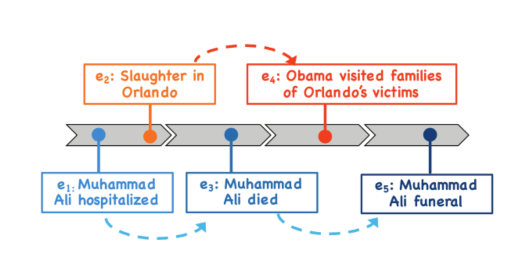
\includegraphics[width=.6\textwidth]{figures/Mele_Muhammad_Ali.png}
    \caption[Two examples of event chains provided by \cite{mele2019event}]{Two examples of event chains provided by \cite{mele2019event}. According to the authors, after event detection, the events are connected ``based on their evolution" (see dashed arrows). However, the algorithm performing this chaining process is not detailed in the paper, and the event chains are absent from annotated data.}
    \label{fig:mele-muhammad}
\end{figure}
%%%%%%%%%%%%%%%%%%%%%%%%%%%%%%%%%%%%%%%%%%%%%%%%%%%%%%%%%%%%%%%%%%%%%%%%%%%%%%%%%%%%%%%

Compared to the previous works reviewed in this section, our contribution is fourfold:
\begin{enumerate}
    \item We propose a new detection method capable of taking into account the temporal evolution of events.
    \item Our approach treats articles from traditional media and Twitter separately at first, so as to preserve distinctive features of Twitter events. The identification of common events is a second step in the process.
    \item We investigate the impact of URLs and hashtags (in addition to word similarity) in joint event detection.
    \item We conduct our experiments on a realistic dataset, which is not only composed of tweets that contain URLs, or tweets from media accounts.
\end{enumerate}
We describe the details of our joint event detection method in the following Section.
\section{Methodology}
Our approach can be broken down into three steps: first, we perform the detection of Twitter events and media events separately. Then we represent the similarity between detected events in a weighted bi-partite graph. Last, we apply a community detection algorithm in order to discover common events accross the two spheres.

\subsection{First Story Detection}
Tweets and news articles are quite different in terms of length and type of vocabulary. Detecting joint events directly from a heterogeneous collection of documents may thus lead to a poor performance (see Section \ref{Joint_results}). In order to let Twitter-specific and media-specific clusters emerge, we thus perform a first event detection step separately for each type of documents. We use the First Story Detection algorithm as described in Algorithm \ref{FSD mini}, which proved to be efficient both on tweets \citep{mazoyer2020french} and news articles \citep{cage2020production}. Since the total number of news articles is much smaller than the number of tweets, we only use mini-batches for tweets, and not for news articles. Second, since words are likely to be used multiple times in each news article, we use the standard tf-idf formulation for news articles representation while we only compute idf for tweets. The formula of idf and tf-idf are given below:
\begin{align}
idf(t) = 1 + log(n+1/df(t)+1)
\end{align}
\begin{align}
tf{\text -}idf(t, d) = tf(t, d) \times idf(t)
\end{align}
where $n$ is the number of documents in the collection, $tf(t, d)$ is the term frequency, \textit{i.e.} the number of times a term $t$ occurs in a document $d$ and $df(t)$ is the document frequency, \textit{i.e.} the number of documents in the collection that contain term $t$.

\subsection{Event-similarity graph}
Once events are detected separately in each sphere, we model the relationships between Twitter events and media events as a weighted bi-partite graph. In the rest of the Chapter, we denote $E_T = \{e_{T,1},\ldots,e_{T,f}\}$ the set of all Twitter events, and $E_M = \{e_{M,1},\ldots,e_{M,g}\}$ the set of all media events. We explore three types of links between Twitter events and media events: word-similarity, URLs and hashtags. 
\paragraph{Word-similarity.}
In order to compute a word-similarity metric between Twitter events and media events, we represent each event as the average of the tf-idf vectors of all documents it contains. The word-similarity between two events is computed as the cosine similarity between these average vectors and used to weight the edge between the two events:
	\begin{equation}
    weight_{text}(e_T, e_M) = \frac{\vec{e_T} \cdot \vec{e_M}}{\| \vec{e_T}\|\| \vec{e_M}\|}
	\end{equation}
Where $\vec{e}$ is the average of the tf-idf vectors of all documents in $e$. To facilitate the community detection step (see Section \ref{Community detection}) , we then remove the edges with a too weak cosine similarity. We denote $s$ the minimum similarity.

\paragraph{Hashtags.} The graph of hashtag relationships between Twitter events and media events is built as follows: if some of the tweets of a Twitter event and some of the articles of a media event have hashtags in common, we draw an edge between the two events. The weight of hashtags is computed as follows:
\begin{equation}
    weight_{htag}(e_T, e_M) = \frac{h(e_T, e_M)}{\max \{h(e_T, e_M): e_T \in E_T,e_M \in E_M \}}
\end{equation}
where $h(e_T, e_M)$ is the number of times the hashtags common to $e_T$ and $e_M$ appear in the Twitter event $e_T$. In order to limit the role of one individual hashtag (e.g. \#BreakingNews) we remove edges where the number of different hashtags is too low.

\paragraph{URLs.} The graph of URLs is constructed in the same way as the graph of hashtags: if tweets within a Twitter event $e_T$ contain an URL pointing to one of the articles in media event $e_M$, we draw an edge between $e_T$ and $e_M$. The weight of urls is computed as follows:
\begin{equation}
    weight_{url}(e_T, e_M) = \frac{u(e_T, e_M)}{\max \{u(e_T, e_M): e_T \in E_T,e_M \in E_M \}}
\end{equation}
where $u(e_T, e_M)$ is the number of times urls linking to articles that are part of media event $e_M$ appear in the tweets of Twitter event $e_T$.

\paragraph{Multidimensional graph.} We combine these three different layers into a single multidimensional graph where the weight of the edges is computed as follows:
\begin{equation}
    weight(e_T, e_M) = \sum_{i \in \{text, url, htag\}} \alpha_i weight_i(e_T, e_M)
\end{equation}
where $0 \leq \alpha_i \leq 1$ and $\sum\limits_{\substack{i \in \{text, url, htag\}}}{\alpha_i = 1}$.

\paragraph{Time of events.} In addition to including word similarity, hashtags and urls in the construction of the event similarity graph, we also take into account the time dimension of the events. We therefore introduce a final parameter, $\Delta$, which indicates the maximum time difference (in days) between a pair of events $(e_T, e_M)$. More precisely, if we call $start$ and $end$ the dates of the first and last document of a given event $e_T$, all media events containing at least one document published between $start - \Delta$ and $end + \Delta$ keep their links with $e_T$ in the graph. Conversely, links between $e_T$ and all other events are removed. Figure \ref{fig:event_time} shows examples of configurations where edges between events are kept, and others where edges are removed.
%%%%%%%%%%%%%%%%%%%%%%%%%%%%%%%%%%%%%%%%%%%%%%%%%%%%%%%
 \begin{figure}
 \begin{center}
      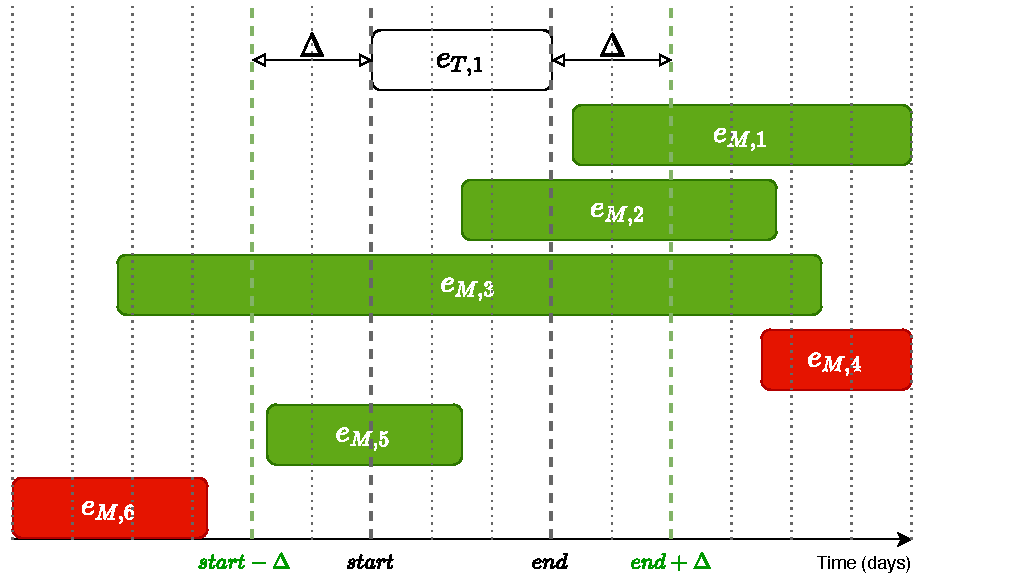
\includegraphics[]{figures/event_time.pdf}
    \caption[Example of different time configurations between a given Twitter event and some media events]{Example of different time configurations between a given Twitter event and some media events. Here the value of parameter $\Delta$ is set to 2 days. Media events ending before $start - \Delta$ or beginning after $end + \Delta$ appear in red. The edges between these events and $e_{T,1}$ are removed in the graph.}
    \label{fig:event_time}
 \end{center}
\end{figure}
%%%%%%%%%%%%%%%%%%%%%%%%%%%%%%%%%%%%%%%%%%%%%%%%%%%%%%

\subsection{Community detection}
\label{Community detection}
Community detection within a network consists in decomposing the network into sub-groups of highly connected nodes. Researchers have proposed many strategies to solve this task, many of them based on the optimization of a given objective function. 

\subsubsection{Modularity}
The most common of these objective functions is the modularity \citep{newman2004finding} of the partition. The aim of this function is to isolate regions of the network where the density of links is higher than expected by chance. Modularity is defined formally  as:
\begin{equation}
    Q = \frac{1}{2m} \sum_{i,j}\left[weight(i,j) - \frac{k_i k_j}{2m}\right]\delta(c_i, c_j)
\end{equation}
where 
\begin{itemize}
    \item $weight(i,j)$ represents the weight of the edge between $i$ and $j$, 
    \item $k_i = \sum\limits_j weight(i,j)$ is the weighted degree of $i$,
    \item $c_i$ is the community to which node $i$ is assigned,
    \item $\delta(x, y)$ is $1$ if $x = y$ and $0$ otherwise, and
    \item $m= \sum\limits_{ij} weight(i,j)$ is the weighted sum of edges.
\end{itemize}
The Louvain algorithm \citep{blondel2008fast} is, to the best of our knowledge, the fastest algorithm to find a partition of the nodes that maximizes modularity. We therefore use this algorithm to identify communities within the event-similarity graph.

\subsubsection{Surprise}
Another metric called surprise \citep{aldecoa_deciphering_2011} outperforms modularity on several benchmarks. It appears to be more efficient when the network contains communities of different sizes, since the modularity metric does not take into account $n_c$ the number of nodes inside a community and $n$ the total number of nodes, in the calculation of the density of links. \cite{traag2015detecting} propose an approximation of surprise in large networks, and an algorithm adapted from the Louvain algorithm, in order to maximize the surprise objective function. Their formulation of the function takes the following form:
\begin{equation}
    Q=mD(q || \hat{q})
\end{equation}
where
\begin{itemize}
    \item $m= \sum\limits_{ij} weight(i,j)$ is the weighted sum of edges,
    \item $q = \frac{\sum\limits_{c}m_c}{m}$ is the fraction of internal edges,
    \item $\hat{q} = \frac{\sum\limits_{c}\binom{n_c}{2}}{\binom{n}{2}}$ is the expected fraction of internal edges, and
    \item $D(x||y) = x \log \frac{x}{y} + (1 - x) \log \frac{1-x}{1-y}$ is the binary Kullback-Leibler divergence.
\end{itemize}
Our event similarity graph is expected to contain a lot of very small communities, containing only one $(e_M, e_T)$ pair. However, in the case of long-lasting events with many sub-events, it is likely that the FSD algorithm over-clusters the events in one of the two spheres (and more likely in tweets). The community detection algorithm should then be able to detect also large communities with many nodes. We therefore also test the algorithm provided by \cite{traag2015detecting}\footnote{\url{https://github.com/vtraag/louvain-igraph}}. We detail our experiments in the next Section.

\section{Experimental Setup}
\subsection{Dataset}
We test our approach on the dataset presented in Chapter 2: it contains 95,796 tweets annotated as related to one of 327 ``daily events" (events were drawn day by day and merged afterwards into 257 ``macro events"). Among these daily events, 296 are actually news articles drawn randomly from a pool of French daily newspapers. The 31 remaining events were detected by monitoring unusually frequent terms on Twitter every day (see Section \ref{Twitter events selection}). We could manually associate 27 of them to a news article from the OTMedia collection \citep{herve2019otmedia}. Concerning the last 4 events, we consider them as purely Twitter events that cannot be merged into a joint event, since we could not find any coverage of these events in traditional media. This makes our dataset all the more realistic: many Twitter events never lead to an article in mainstream media.

We ran the FSD algorithm on the OTMedia collection in order to automatically group the selected articles with other articles adressing the same topics. From these 323 articles (296 + 27), 167 were automatically clustered with other articles from our pool. In total, we obtained 15,544 news articles from 61 media outlets. We are aware that automatically grouping articles using the FSD algorithm may bias the dataset in favour of our approach, since part of it relies on the FSD algorithm. In order to prove the validity of our approach, we therefore systematically present two type of results: first, results computed on the entire dataset, second, results computed only on tweets (that were entirely manually annotated and are therefore not biased).

\subsection{Evaluation metric}
In an approach similar to that of Chapter 3 (see Section \ref{metric_best_matching}), we evaluate the performance of our algorithm using the ``best matching" precision, recall and F1 score \citep{yang1998study} for each event in the ground truth. We then compute the average of the events, to provide a macro-average result.

\subsection{Parameter tuning}

In the first step of our approach (First Story Detection applied on tweets and news articles separately), we use the same parameters as \cite{cage2020production} for news articles (threshold $t$ of $0.67$ and time window $w$ of one day), and the best parameters found in  \cite{mazoyer2020french} (see Section \ref{Subsec: text embeddings}: $t=0.7$ and $w$ set to one day) for tweets.

The graph construction step of our method requires many different parameters, leading to a risk of over-fitting. To test the robustness of our model on different samples, we divide our dataset in 4 sub-samples of equal number of documents. The FSD algorithm requires documents to be sorted in chronological order, this is why we do not select documents randomly: we split the dataset in 4 different time periods and test each combination of parameters on each subset. We present the role of the different parameters in the next Section.

\section{Results}

We observe a small effect of the choice of the community detection quality metric on the results of our model: surprise outperforms modularity in all cases, however not significantly (see Figures \ref{fig:louvain_macro_days} and \ref{fig:louvain_macro_sim}). Regarding the choice of parameters, they tend to have similar effects on each subset of our evaluation corpus. We analyze the role of each parameter more in depth in the rest of this section. We first detail the contribution of the different modalities of event similarity (word similarity, URLs, hashtags). We then present the best choice of $\Delta$ and $s$ parameters.

\subsection{Effect of word similarity, URLs and hashtags}
Figure \ref{fig:louvain_macro} shows 
the best configuration of parameters $\alpha_{text}$, $\alpha_{url}$, $\alpha_{htag}$ and $\Delta$ for each subset, with other parameters being fixed ($s = 0.3$ and $l = 3$). Overall, the results are quite stable to the change of parameters, even if the model performs better on all subsets when the weight of word-similarity ($\alpha_{text}$) is high. URLs and hashtags seem to have a much lower effect, particularly when evaluating the model only on tweets (Figure \ref{fig:louvain_macro_tweets}). Increasing $\alpha_{url}$ or $\alpha_{htag}$ may slightly improve the performance on some time periods  but there is no configuration that performs equally well on each subset.

  We therefore chose to eliminate these modalities, in order to simplify the graph construction step and to obtain a model that is more stable to the change of dataset. We show the results with a model relying on text only in the right column of Figures \ref{fig:louvain_macro_all} and \ref{fig:louvain_macro_tweets}. The low effect of URLs and hashtags can be explained by the fact that the information carried by these modalities is in most cases already present in the text of the documents.
%%%%%%%%%%%%%%%%%%%%%%%%%%%%%%%%%%%%%%%%%%%%%%%%%%%%%%%
 \begin{figure}
 
 \begin{subfigure}[b]{1\textwidth}
    \begin{center}
      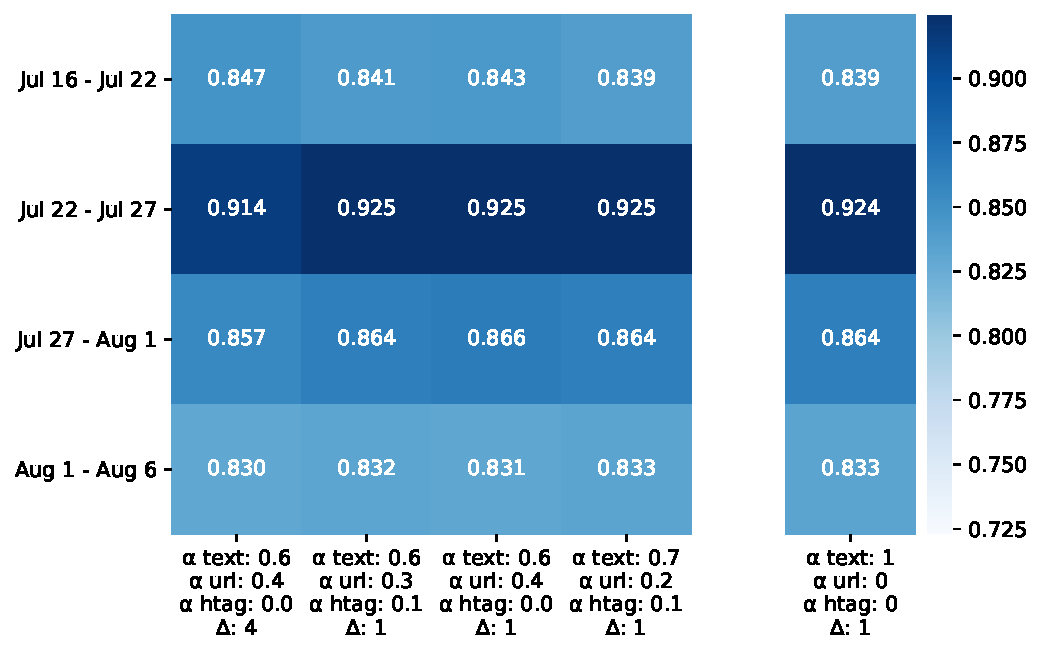
\includegraphics[height=.4\textheight]{figures/louvain_macro_tfidf.pdf}
    \caption{Evaluation on all documents}
    \label{fig:louvain_macro_all}
    \end{center}
\end{subfigure}
\begin{subfigure}[b]{1\textwidth}
\begin{center}
 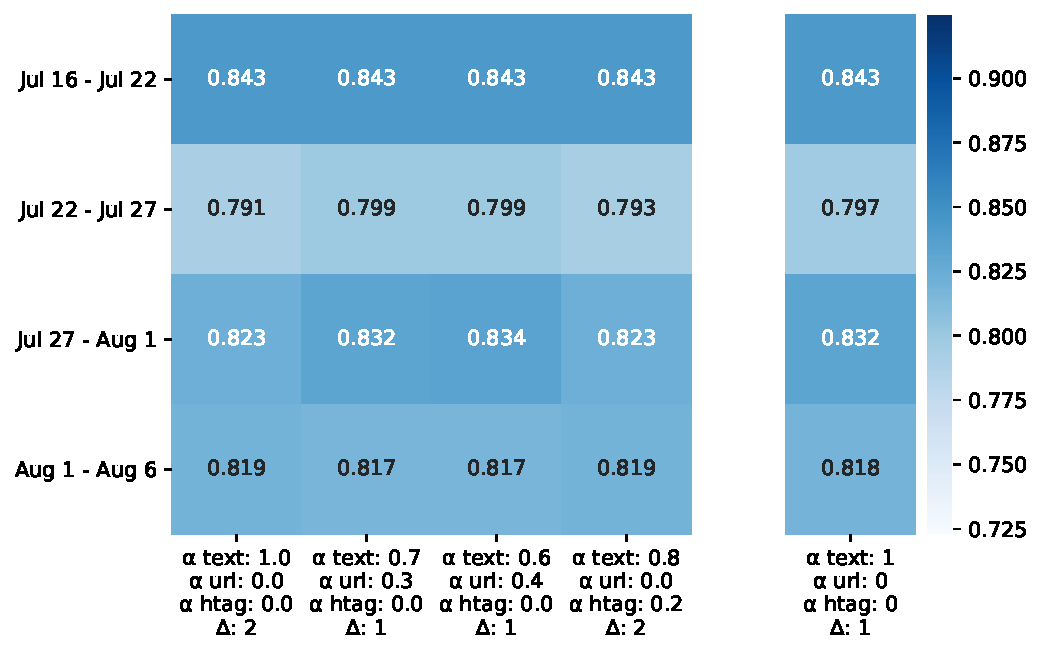
\includegraphics[height=.4\textheight]{figures/louvain_macro_tfidf_tweets_only.pdf}
       \caption{Evaluation on tweets only}
    \label{fig:louvain_macro_tweets}
     \end{center}
\end{subfigure}
\caption[Best matching F1 score of our approach on different sub-samples]{Best matching F1 score of our approach on different sub-samples. The result of community detection with the best set of parameters for a given sample is displayed on the diagonal of the square matrix. The results of that set of parameters on the other samples are displayed on the corresponding lines. The right column presents the results of community detection on the word-similarity graph only (urls and hashtags are not taken into account). The other parameters are fixed: $s=0.3$, $l=3$}
\label{fig:louvain_macro}
\end{figure}

\subsection{Effect of the maximum time distance between 2 events ($\Delta$)}
Figure \ref{fig:louvain_macro_days} presents the average F1 score of our model on the 4 subsets depending on the value of $\Delta$, all other parameters being fixed. We observe little impact of that variable, with a slightly better performance when $\Delta=1$. However, each subset contains less than 6 days of data, a period during which it is unlikely that two semantically close nodes actually belong to two different joint events. 

%%%%%%%%%%%%%%%%%%%%%%%%%%%%%%%%%%%%%%%%%%%%%%%%%%%%%
\begin{figure}
    \centering
    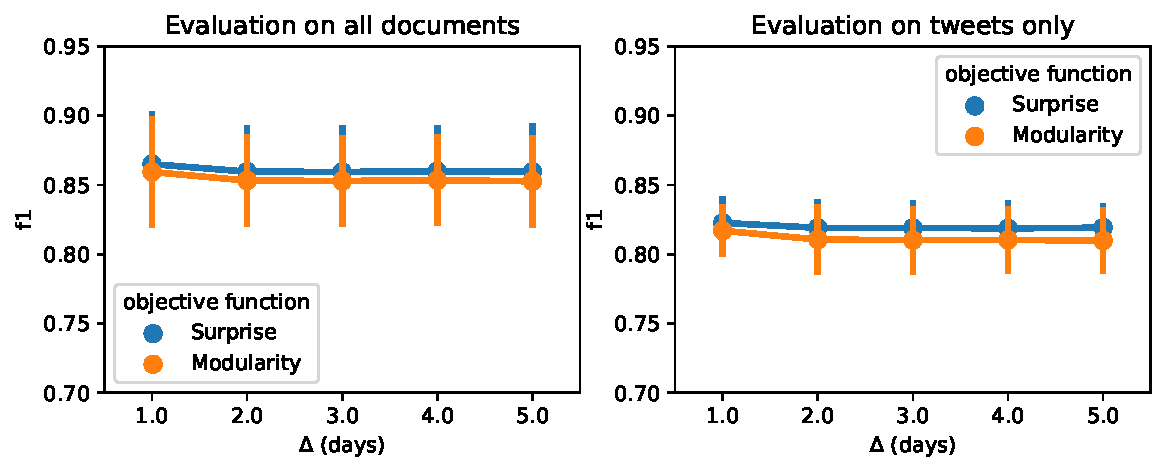
\includegraphics[width=1\textwidth]{figures/louvain_macro_days.pdf}
    \caption[Effect of the of the maximum time distance on the performance of our method]{Effect of the of the maximum time distance ($\Delta$) on the performance of our method. This Figure plots the average best matching F1 score for the 4 subsets, with standard deviation, depending on $\Delta$.}
    \label{fig:louvain_macro_days}
\end{figure}
%%%%%%%%%%%%%%%%%%%%%%%%%%%%%%%%%%%%%%%%%%%%%%%%%%%%%
\subsection{Effect of the minimum cosine similarity between 2 events ($s$)}
Figure \ref{fig:louvain_macro_sim} shows the average performance of our approach on each subset depending on the value of $s$. The optimal value of $s$ is $0.3$. The choice of the objective function has a real impact for low values of $s$, i.e. when practically all edges are kept in the event-similarity graph. It appears that the surprise function gives better results when the number of edges increases. However, for $s=0.3$ and higher, the choice of the quality function makes no difference.

%%%%%%%%%%%%%%%%%%%%%%%%%%%%%%%%%%%%%%%%%%%%%%%%%%%%%
\begin{figure}
    \centering
    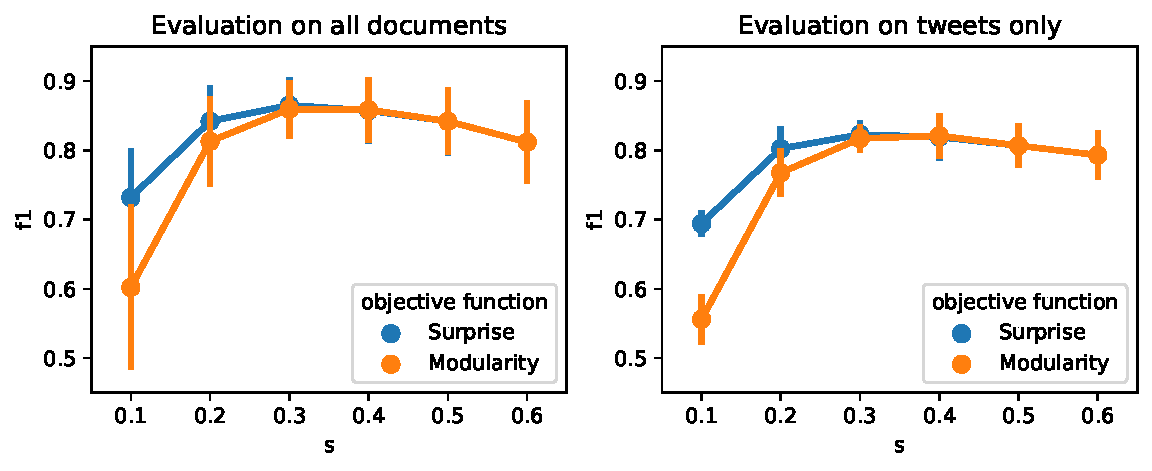
\includegraphics[width=1\textwidth]{figures/louvain_macro_sim.pdf}
    \caption[Effect of the minimum cosine similarity between 2 events on the performance of our method.]{Effect of the minimum cosine similarity between 2 events ($s$) on the performance of our method. This Figure plots the average best matching F1 score for the 4 subsets, with standard deviation, depending on $s$.}
    \label{fig:louvain_macro_sim}
\end{figure}
%%%%%%%%%%%%%%%%%%%%%%%%%%%%%%%%%%%%%%%%%%%%%%%%%%%%%
\subsection{Results on the entire corpus}
\label{Joint_results}

\section{Conclusion}
